\begin{abcliste}
\abc
\begin{center}
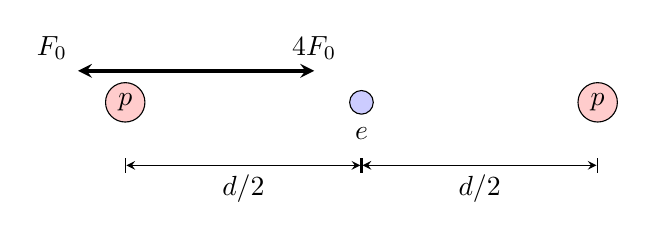
\begin{tikzpicture}[>=stealth]
 \draw[fill=red!20] (0,0) circle (0.25) node {$p$};
 \draw[fill=blue!20] (3,0) circle (0.15) node[below=2mm] {$e$};
 \draw[fill=red!20] (6,0) circle (0.25) node {$p$};
 \draw[|<->|] (0,-0.8) -- node[below] {$d/2$} (3,-0.8);
 \draw[|<->|] (3,-0.8) -- node[below] {$d/2$} (6,-0.8);
 \draw[->, very thick] (0,0.4) -- (2.4,0.4) node[above] {$4F_0$};
 \draw[->, very thick] (0,0.4) -- (-0.6,0.4) node[above left] {$F_0$};
\end{tikzpicture}
\end{center}
Consider the left proton. The other proton, at the distance $d$, repels it with
\begin{align}
 F_0 &= \FzF = \kC\times\frac{\left(\qe\right)^2}{\left(\dh\right)^2} = \Fz
\end{align}
The electron, at the distance $d/2$, attracts it with $k\,e^2/(d/2)^2 = 4\,F_0$. Both forces lie on the line through the particles, in opposite directions:
\begin{align}
 F &= 4\,F_0 - F_0 = \FF \\
   &= 3\times\Fz \\
   &= \F \approx \result{\FP{-9}{2}}
\end{align}
It points \emph{towards the electron}: the electron holds the molecule together. The same holds for the right proton, by symmetry.

\abc The electron is attracted by both protons equally strongly, from the same distance $d/2$, but in opposite directions: the two forces cancel.
\end{abcliste}
